\documentclass[11pt]{amsart}
\usepackage{amsmath,amssymb,amsthm,mathtools,enumitem}
\usepackage[margin=1in]{geometry}
\usepackage{hyperref}
\usepackage{graphicx}
\graphicspath{{./}{../figures/}}

\newtheorem{theorem}{Theorem}[section]
\newtheorem{proposition}[theorem]{Proposition}
\newtheorem{corollary}[theorem]{Corollary}
\theoremstyle{remark}
\newtheorem*{remark}{Remark}

\title{The Cutting Plane: Every Line Through the Multiplication Table Is a Conic Section}
\author{Jeremy Ebert}
\address{Franklin County, Ohio, USA}
\date{2026}

\begin{document}
\maketitle

\begin{abstract}
Write out the ordinary multiplication table and draw a straight line through it. What curve does that line trace, once factor pairs are plotted in coordinates built from their sum, difference, and geometric mean? We classify the resulting sections completely: ellipse, parabola, hyperbola, or the degenerate generator case according to the line coefficients. Anti-diagonals give circles and individual rows or columns give parabolas. We also isolate an exact tangency between every row/column parabola and the anti-diagonal circle whose diameter equals the fixed factor level, and give the true semi-axes and eccentricity of the general ellipse section. The same coordinates restate Fermat factorization and reorganize the classical Dirichlet divisor summatory identity around nested diagonal gnomons.
\end{abstract}

\section{Introduction}
Figure~\ref{fig:table_line}(b) is the ordinary multiplication table written in the coordinates
\[
X=\frac{x-y}{2},\qquad T=\frac{x+y}{2}.
\]
Every lattice cell still represents the ordinary product $xy$; the coordinate change merely turns the usual square arrangement into a triangular side view. The outer boundary shown is $x+y=12$, and the dashed anti-diagonal $x+y=8$ passes through $(2,6),(4,4),(6,2)$.

There is also a classical geometric reason for the third coordinate. Given a rectangle with sides $x$ and $y$, place the two lengths end to end as the diameter of a semicircle and erect the perpendicular at their junction. The right-triangle altitude theorem gives that perpendicular length as $\sqrt{xy}$. If
\[
Y=\sqrt{xy},\qquad T=\frac{x+y}{2},\qquad X=\frac{x-y}{2},
\]
then the radius, altitude, and signed offset form a right triangle and therefore satisfy
\[
X^2+Y^2=T^2.
\]
Thus every positive factor pair lies on the cone in Figure~\ref{fig:table_line}(c). For example, $(x,y)=(2,6)$ gives $(X,Y,T)=(-2,\sqrt{12},4)$ and $4+12=16$.

Anti-diagonals $x+y=K$ become fixed-$T$ circles. A general line $ax+by=c$ becomes a cutting plane, and its intersection with the cone is a conic section. The reflected pair
\[
8x+4y=32,\qquad 4x+8y=32
\]
is shown throughout Figure~\ref{fig:table_line} as a concrete example.

The emphasis here is deliberately geometric and elementary. Arithmetic structures that can subsequently act on this cone are treated in companion work; none is required for the results below.

\begin{figure}[ht]
\centering
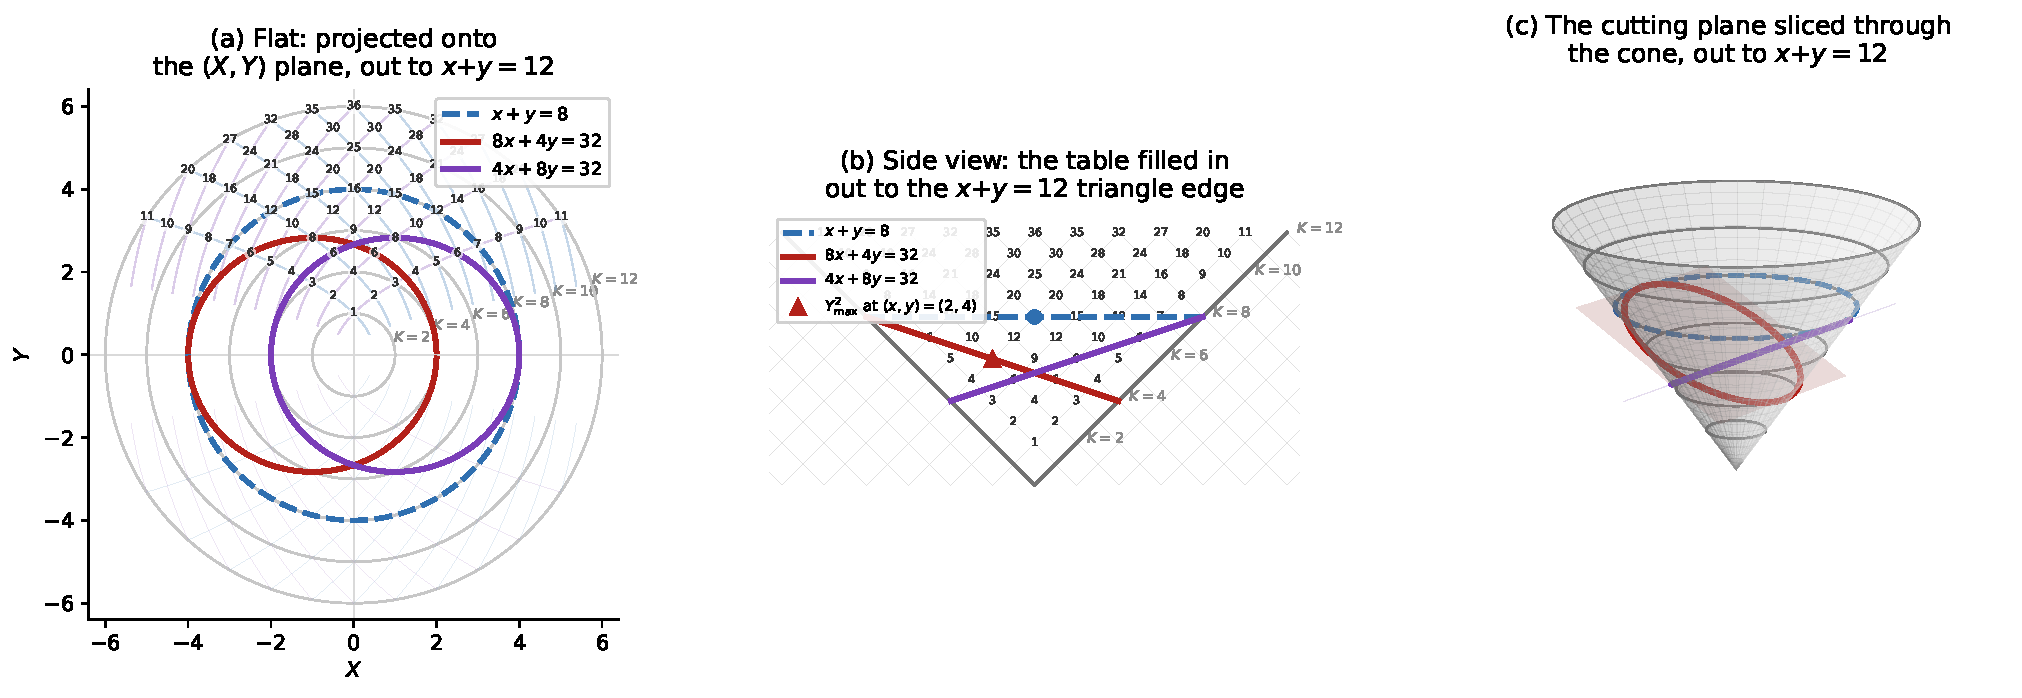
\includegraphics[width=\textwidth]{fig_cutting_plane_3panel.pdf}
\caption{Three views of the same factor geometry, bounded by $x+y=12$. (a) Fixed sums are concentric circles, row and column families are mirror parabolas, and the red/purple cuts are the mirror ellipses from $8x+4y=32$ and $4x+8y=32$. (b) Side view in $(X,T)$, where the multiplication table becomes a triangular lattice. (c) The same cuts as literal plane sections of $X^2+Y^2=T^2$. The figure is illustrative; the claims are proved below.}
\label{fig:table_line}
\end{figure}

\section{Mean-Value Coordinates and the Conic Identity}
For $x,y>0$ define
\begin{equation}
X=\frac{x-y}2,\qquad Y=\sqrt{xy},\qquad T=\frac{x+y}2. \tag{2.1}
\end{equation}
Then
\begin{equation}
X^2+Y^2=T^2. \tag{2.2}
\end{equation}
The inverse factor coordinates are
\begin{equation}
x=T+X,\qquad y=T-X. \tag{2.3}
\end{equation}
Thus factor exchange $(x,y)\mapsto(y,x)$ is exactly $X\mapsto-X$ with $Y,T$ fixed. We use this convention throughout; in particular positive $X$ means $x>y$.

Fixing $x+y=K$ fixes $T=K/2$, giving the circle
\[
X^2+Y^2=(K/2)^2.
\]
For integer $K\ge2$, the positive factor lattice contributes the $K-1$ points $(x,K-x)$, $x=1,\ldots,K-1$, to this circle.

\begin{remark}[Area is not preserved]
Although $Y^2=xy$ records the area of the factor rectangle as a scalar, the map $(x,y)\mapsto(X,Y,T)$ is not area-preserving on the cone. In particular, one should not identify the Euclidean surface area of a cone patch with the area $xy$ of the corresponding multiplication-table cell. The exact flat Jacobian, induced cone-area factor, band areas, hyperbola/secant partition, and the weighted inverse measure in circle coordinates are treated separately in the companion note \cite{Ebert2026Area}; no area-preservation statement is used in this paper.
\end{remark}

\section{The General Conic Theorem}
\begin{theorem}\label{thm:conic}
Let $a,b$ be real numbers, not both zero, and let $ax+by=c$ meet the positive factor quadrant. On the full algebraic cone section, the cut is an ellipse when $ab>0$, a parabola when $ab=0$, and a nondegenerate hyperbola when $ab<0$ and $c\ne0$. When $ab<0$ and $c=0$, the section degenerates into the pair of cone generators in the full double-cone picture; within the positive-factor branch only one generator ray is present. When $a=b\ne0$, the ellipse is a fixed-sum circle.
\end{theorem}
\begin{proof}
For $b\ne0$, $y=(c-ax)/b$, hence
\[
Y^2=xy=\frac cbx-\frac abx^2.
\]
If $ab>0$, the coefficient of $x^2$ is negative and the positive-quadrant section is an ellipse. The cases $a=0$ or $b=0$ are the row/column parabolas below. If $ab<0$ and $c\ne0$, the quadratic has the nondegenerate hyperbolic sign. If $ab<0$ and $c=0$, then
\[
Y^2=-\frac abx^2,
\]
which factors into two straight generators in the full algebraic section; the positive-factor branch retains the ray compatible with $x,y\ge0$. If $a=b\ne0$, then $x+y=c/a$ is constant.
\end{proof}

\begin{proposition}[Rows and columns]\label{prop:rows}
With the convention $X=(x-y)/2$, a fixed row $x=u$ satisfies
\[
X+T=u,\qquad Y^2=u(T-X)=u^2-2uX,
\]
while a fixed column $y=u$ satisfies
\[
T-X=u,\qquad Y^2=u(T+X)=u^2+2uX.
\]
The two projected parabolas are exchanged by $X\mapsto-X$.
\end{proposition}

\begin{proof}
For $x=u$, equations (2.3) give $T+X=u$ and $y=T-X$, hence $Y^2=xy=u(T-X)$. The column identity is the factor-exchange reflection. In three dimensions the row plane $T+X=u$ is parallel to the cone generator $(-1,0,1)$, and the column plane $T-X=u$ is parallel to $(1,0,1)$, giving the classical plane-section characterization of a parabola.
\end{proof}

\begin{proposition}[Anti-diagonal tangency]\label{prop:tangent}
For every $u>0$, the row and column parabolas at factor level $u$ are tangent in the $(X,Y)$ projection to
\[
C_{u/2}:\quad X^2+Y^2=(u/2)^2.
\]
The row $x=u$ is tangent at $(X,Y)=(u/2,0)$, and the column $y=u$ at $(-u/2,0)$. On the cone these are $(T,X,Y)=(u/2,\pm u/2,0)$.
\end{proposition}
\begin{proof}
The row parabola $Y^2=u^2-2uX$ has vertex $(u/2,0)$; the column parabola $Y^2=u^2+2uX$ has vertex $(-u/2,0)$. Both vertices lie on $C_{u/2}$, and implicit differentiation gives the same vertical tangent there. The signs also follow directly from (2.3): at the row endpoint $y=0$, $X=x/2=u/2$; at the column endpoint $x=0$, $X=-y/2=-u/2$.
\end{proof}

\begin{remark}
Factor level $u$ corresponds exactly to tangent-circle radius $T=u/2$. A factor mesh of spacing $1/m$ therefore induces a tangent-circle radius mesh of spacing $1/(2m)$. This is a geometric statement, not an arithmetic invariance claim.
\end{remark}

For the metric statements about an ellipse, multiplying the line equation by $-1$ if necessary lets us normalize the nonempty positive-quadrant case to $a,b,c>0$ without changing the geometric line.

\begin{proposition}[Coordinate maximum of an ellipse]\label{prop:semiaxes}
Assume $a,b,c>0$. Then $Y^2$ is maximized at
\[
x=\frac{c}{2a},\qquad y=\frac{c}{2b},
\]
and
\[
Y_{\max}^2=\frac{c^2}{4ab}.
\]
\end{proposition}
\begin{proof}
Differentiate $Y^2=(c/b)x-(a/b)x^2$ and substitute the critical point; the line equation then gives the stated $y$ coordinate.
\end{proof}

For $8x+4y=32$, the maximum is $(x,y)=(2,4)$ with $Y^2_{\max}=8$. Since $X=(x-y)/2$, this point has $(X,T)=(-1,3)$. Its reflected cut $4x+8y=32$ has maximum $(4,2)$ and $(X,T)=(1,3)$. This fixes the red/purple orientation independently of the drawing.

\begin{proposition}[True ellipse axes and eccentricity]\label{prop:trueaxes}
Assume $a,b,c>0$. The ellipse cut from the cone by $ax+by=c$ has semi-minor axis
\[
b_{\rm semi}=\frac{c}{2\sqrt{ab}},
\]
semi-major axis
\[
a_{\rm semi}=\frac{c\sqrt{2(a^2+b^2)}}{4ab},
\]
and eccentricity
\[
e=\frac{|a-b|}{\sqrt{a^2+b^2}}.
\]
Thus eccentricity depends only on $a/b$, and $e=0$ exactly when $a=b$.
\end{proposition}
\begin{proof}
The section is symmetric under $Y\mapsto-Y$, and the $Y$ direction lies in the cutting plane. Its $Y$ semi-axis is therefore $Y_{\max}=c/(2\sqrt{ab})$. At $Y=0$ the two endpoints are
\[
\left(\frac{c}{2a},0,\frac{c}{2a}\right),\qquad
\left(-\frac{c}{2b},0,\frac{c}{2b}\right).
\]
The direction joining these endpoints is orthogonal to the $Y$ direction, so half their Euclidean distance is the other semi-axis, namely
\[
\frac{c\sqrt{2(a^2+b^2)}}{4ab}.
\]
Moreover
\[
\frac{a_{\rm semi}^2}{b_{\rm semi}^2}=\frac{a^2+b^2}{2ab}\ge1,
\]
so these are indeed the major and minor axes. Finally $e^2=1-b_{\rm semi}^2/a_{\rm semi}^2=(a-b)^2/(a^2+b^2)$.
\end{proof}

For $8x+4y=32$,
\[
a_{\rm semi}=\sqrt{10},\qquad b_{\rm semi}=2\sqrt2,\qquad e=1/\sqrt5.
\]
The standard circumference formula is therefore also available as $C=4a_{\rm semi}E(e)$, where $E$ denotes the complete elliptic integral of the second kind; we do not otherwise use it here.

\section{Constant-Product Curves and Fermat Factorization}
Fixing $xy=N$ fixes $Y^2=N$, so
\begin{equation}
T^2-X^2=N. \tag{4.1}
\end{equation}
For odd $N$, Fermat's method searches integers $T\ge\lceil\sqrt N\rceil$ until $T^2-N=X^2$, at which point
\[
N=(T-X)(T+X).
\]
Thus the constant-product hyperbola records the same factorization search directly in mean-value coordinates.

\section{The Divisor Summatory Function via Nested Gnomons}
Let
\[
D(n)=\sum_{k=1}^n d(k)=\#\{(x,y)\in\mathbb Z_{\ge1}^2:xy\le n\}.
\]
For each diagonal vertex $(u,u)$, $1\le u\le\lfloor\sqrt n\rfloor$, the horizontal and vertical arms terminate at the constant-product boundary. Their integer arm length is $\lfloor n/u\rfloor-u$. Hence
\begin{equation}
D(n)=\sum_{u=1}^{\lfloor\sqrt n\rfloor}\left[2\left(\left\lfloor\frac nu\right\rfloor-u\right)+1\right], \tag{5.1}
\end{equation}
and therefore
\begin{equation}
D(n)=2\sum_{u=1}^{\lfloor\sqrt n\rfloor}\left\lfloor\frac nu\right\rfloor-\lfloor\sqrt n\rfloor^2. \tag{5.2}
\end{equation}
This is the classical symmetric Dirichlet hyperbola identity, read as nested gnomons whose arms are pieces of the row/column parabolas cut off by $xy=n$.

For $n=11$, the smallest integer anti-diagonal bounding the whole positive divisor region is $x+y=12$. The triangular region
\[
x+y\le12
\]
contains
\[
T_{11}=1+2+\cdots+11=66
\]
positive lattice cells. Within that triangle,
\[
D(11)=29,\qquad A_{11}:=T_{11}-D(11)=37.
\]
The constant-product boundary is
\[
xy=11\iff Y=\sqrt{11}\iff T^2-X^2=11,
\]
and it meets $x+y=12$ at $(1,11)$ and $(11,1)$, corresponding to $(X,T)=(-5,6)$ and $(5,6)$.

\begin{figure}[ht]
\centering
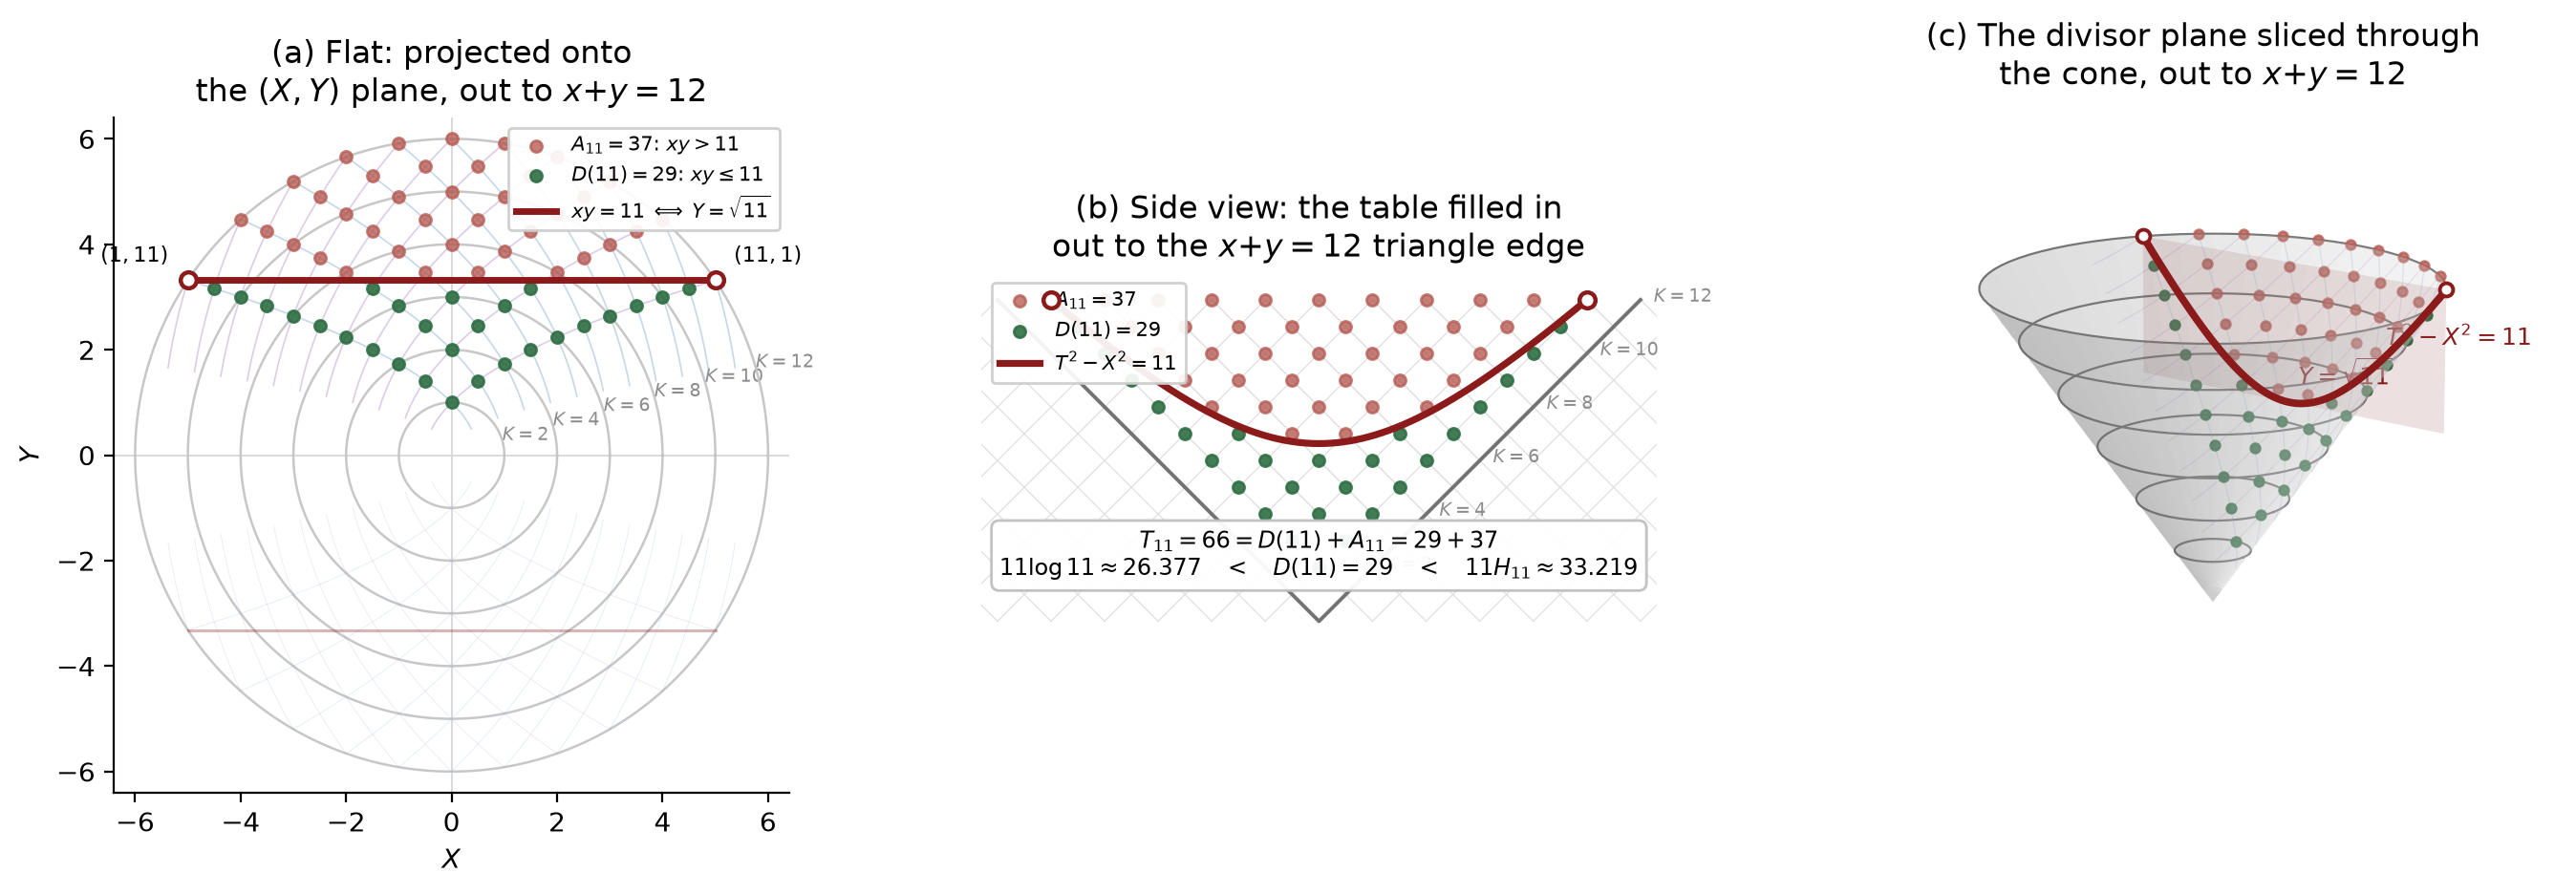
\includegraphics[width=\textwidth]{fig_divisor_summatory_11_3panel.png}
\caption{The divisor summatory geometry for $n=11$ in the same three views as Figure~\ref{fig:table_line}. The $66$ cells inside $x+y\le12$ split exactly into $D(11)=29$ and the triangular complement $A_{11}=37$. The boundary $xy=11$ is $Y=\sqrt{11}$ in the flat projection, $T^2-X^2=11$ in the side view, and the section by the vertical plane $Y=\sqrt{11}$ in three dimensions. The displayed $11\log11$ and $11H_{11}$ values are comparison quantities only; they are not asserted to equal the discrete count.}
\label{fig:divisor11}
\end{figure}

The choice $n=11$ is illustrative rather than structural: the identities above hold for general $n$. It is useful here because the extremal factor pairs lie exactly on $x+y=12$.

\section{Discussion}
The cone identity organizes three elementary structures on one carrier: linear conditions become conic sections, constant products become Lorentz-type hyperbolas, and the divisor summatory region decomposes into diagonal gnomons. Proposition~\ref{prop:tangent} adds an exact bridge: each fixed factor level determines both a row/column parabola and a unique tangent anti-diagonal circle of radius $u/2$.

The sign convention is fixed globally by $X=(x-y)/2$: rows terminate on the positive-$X$ generator, columns on the negative-$X$ generator, and factor exchange is reflection through $X=0$. Figures~\ref{fig:table_line} and~\ref{fig:divisor11} use this same convention.

At the coarsest finite level, an integer factor pair also has an elementary four-state reduction: reducing $(x,y)$ modulo $2$ gives $(\epsilon_1,\epsilon_2)\in\mathbb F_2^2$, factor exchange swaps the two coordinates, and the parity $\epsilon_1\oplus\epsilon_2$ is invariant under that exchange. This observation uses only the factor-coordinate cell itself; no cyclotomic, ideal-theoretic, or operator interpretation is needed here.

This is the natural stopping point for the geometric paper. Later arithmetic or operator constructions may use the same cone and its two generator rays, but they should be cited as companion results rather than imported into these elementary proofs.

\begin{thebibliography}{9}
\bibitem{Dickson} L.~E.~Dickson, \emph{History of the Theory of Numbers, Vol.~I}, Carnegie Institution, 1919, Ch.~14.
\bibitem{Dirichlet} P.~G.~L.~Dirichlet, \"Uber die Bestimmung der mittleren Werthe in der Zahlentheorie, \emph{Abh. K\"onigl. Preuss. Akad. Wiss.} (1849), 69--83.
\bibitem{Ebert2026Area} J.~Ebert, \emph{Area Distortion and Exact Band Geometry of the AM--GM Cone}, preprint (2026).
\end{thebibliography}
\end{document}
